\appendix
  \textbf{\huge{Appendice}}
  \section{Tavola di verità di 1-bit full adder}\label{sec:1bfa-tavola}
  tabella
  \section{Schema del circuito di 1-bit full adder}\label{sec:1bfa-circuito}
    \begin{figure}[h]
      \centering
      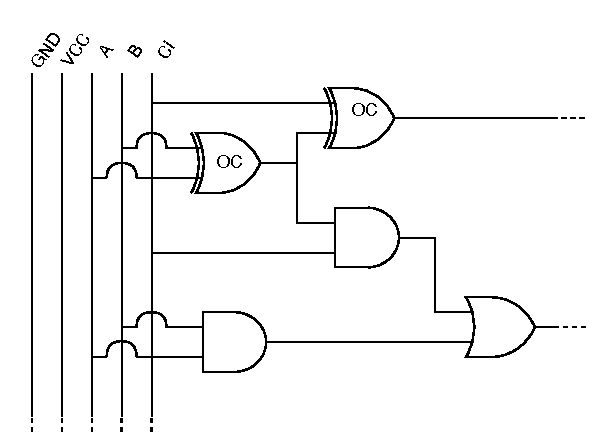
\includegraphics[width=10cm]{../assets/1bfa.drawio.pdf}
      \caption{
        \emph{
          Schema del circuito 1-bit full adder. Le iniziali "\textsc{oc}" sui gate \textsc{xor} indicano che i gate sono
          \emph{open collector}.
        }
      }
      \label{fig:circuito}
    \end{figure} %todo
